\chapter{Generalized Bayesian Inference with Sets of Priors}

\begin{itemize}
\item Short introduction to IP (sets of priors, lower/upper prevision/probability)
%\item motivate imprecise priors with ress paper: \cite{Troffaes2013a} --- now in intro
\item \pdc\ (Evans \& Moshonov, Fuquene-Cook-Pericchi), examples (Festschrift paper: \cite{Walter2010a})
\item further motivations for IP (ITIP chapter \cite{itip-statinf}) 
\item Generalized Bayesian inference
\item Generalized Bayesian inference with sets of priors
 \begin{itemize}
 \item sets of priors, GBR, robust Bayes
 \item sets of conjugate priors in general
 \item parameter set shapes
 \end{itemize}
\item IDM
\item JSTP paper \cite{Walter2009a}
\item isipta11 paper \cite{Walter2011a}
\item boatshape?
\end{itemize}

After having seen a detailed example for Bayesian inference using sets of conjugate priors in Section~\ref{sec:commoncause},
in the main chapter of this thesis,
we will give now a general introduction to the methodology of Bayesian inference with sets of conjugate priors.
In Section ****, \\
Section **** 


\section{Imprecise or Interval Probability}
\label{sec:ip-intro}

This Section will give a condensed introduction to the main theoretic concepts
in interval or imprecise probability as needed for the topics discussed in this thesis.

While Section~\ref{sec:ip-general} follows mostly \textcite{2011:IESS-ip},
Section~\ref{sec:ip-main} is based mainly on \textcite{1996:walley::expert} and \textcite{2000:walley::towards}.


\subsection{General Concept and Basic Interpretation}
\label{sec:ip-general}

The central idea of imprecise or interval probability \parencite{2011:IESS-ip, 1991:walley, 2001:weichselberger} is
to replace the usual, precise probability measure $\p(A)$ for events $A$%
\footnote{Events of interest $A$ are taken to be subsets of the sample space $\Omega$,
forming a $\sigma$-algebra, a non-empty collection of sets including countable unions and intersections of subsets of $\Omega$.}
with a \emph{lower} and \emph{upper probability}, denoted by $\Pl(A)$ and $\Pu(A)$, respectively,
satisfying
\begin{equation}
\label{eq:0ip1}
0 \le \Pl(A) \le \Pu(A) \le 1\,.
\end{equation}
In this setting, a usual probability measure forms the extreme case $\Pl(A) = \Pu(A) = \p(A)$,
when there is enough information to determine the distribution on the sample space $\Omega$
in precise stochastic terms.
On the other extreme, when $\Pl(A) = 0$ and $\Pu(A) = 1$,
we have no information at all on the probability for $A$ to occur,
and intermediate cases $0 \le \Pl(A) < \Pu(A) \le 1$ represent
different degrees of knowledge on this probability.

Therefore, interval or imprecise probability adds another modeling dimension:
While usual, precise probability measures can be used to model phenomena when there is perfect stochastical information,
like, e.g., in a lottery where the number of winning tickets (and the total number of tickets) is precisely known,
imprecise probability measures can account for cases where there is uncertainty about the probabilities themselves,
just like in a lottery where the number of winning tickets is not exactly known.
Non-stochastic uncertainty about model features like probabilities is often called \emph{ambiguity},
forming a crucial part of the human decision process,
and there are studies suggesting that humans process ambiguity in a way
differing from pure probabilistic reasoning \parencite{2005:hsu-bhatt}.

In contrast to a probability measure $\p(A)$,
the set functions $\Pl(A)$ and $\Pu(A)$ do not adhere
to the additivity axiom of Kolmogorov's \parencite*{1933:kolmogorov}
formalization of probability as a normed measure,
%(countable or finite additivity),
and thus are also known as \emph{non-additive probabilities}.
There is also a link to \emph{fuzzy measures}, which are also non-additive measures
\parencite[see, e.g.,][]{1997:denneberg}.

In general, $\Pl(A)$ may be understood as accounting for evidence certainly in favour of $A$,
and $\Pu(A)$ accounting for all evidence speaking not strictly against $A$.
The difference of $\Pu(A)$ and $\Pl(A)$ thus allows for inconclusive evidence
that may not speak unanimously in favor of or against $A$, respectively.
As evidence strictly against $A$ can be seen as evidence certainly in favour of $A^\com$,
the complement of $A$,
it is mostly assumed that $\Pl(A^\com) = 1 - \Pu(A)$,
and thus it suffices to determine either of $\Pl$ or $\Pu$,
the other one being defined through this relation.

There are currently two main approaches to a general theory of statistical inference with interval or imprecise probability:
\begin{enumerate}[(i)]
\item The theory by \textcite{2000:weichselberger, 2001:weichselberger}
regards probability intervals $[\Pl(A), \Pu(A)]$ for all or some events $A$ as the basic entity
\parencite[p.~646]{2011:IESS-ip},
from which an interval-valued distribution on the sample space $\Omega$ is constructed.
His approach is axiomatic, in the sense that it replaces Kolmogorov's \parencite*{1933:kolmogorov} additivity axiom by two axioms,%
\footnote{The first states that \eqref{eq:0ip1} holds,
the second that the set $\mathcal{M}$ consisting of all usual, precise distributions $\p(\cdot)$
with $\Pl(A) \le \p(A) \le \Pu(A)$, for all $A \in \Omega$, is non-empty.
The second axiom guarantees that there exists at least one precise probability distribution
which is compatible with an interval-valued probability distribution,
and thus rules out the case of contradictory assignments of $[\Pl(A), \Pu(A)]$.}
from which the theory is derived,
while imposing no specific interpretation on these constructs.
This theory of interval probability was developed
as the foundation of a concept of \emph{logical probability} \parencite{2007:weichselberger},
where probability is not assigned to events, but to logical conclusions (from a premise to a consequence),
with the aim to arrive at a theory of statistical inference
which allows for fiducial-like probability statements,
e.g., probability statements on parameters similar to a posterior distribution in a Bayesian setting
without the need to specify a prior distribution \parencite{2011:IESS-fiducial}.
\item In contrast, the theory by Walley \parencite*{1991:walley, 2000:walley::towards}
aims to generalise the Bayesian approach to statistical inference,
adopting a strictly subjective interpretation for imprecise probability
as lower and upper betting rates (see below),
and extending the Bayesian paradigm (as discussed in Section~\ref{sec:bayes-inference})
to imprecise probability distributions.
In generalising de Finetti \parencite*{1937:finetti,1970:finetti}, the basic entities are lower and upper \emph{previsions},
i.e.\ expectation functionals, for \emph{gambles}, i.e.\ random variables,
instead of lower and upper probabilities for events.
This is due to the fact that unlike in precise probability theory%
---where the definition of a distribution via expectations %precise previsions
(often denoted \emph{linear previsions} in the imprecise probability literature)
is eqivalent to a definition via a precise probability distribution---%
the definition of an imprecise distribution via lower and upper previsions
is more general than a definition via lower and upper probability for events
\parencite[p.~132]{2000:walley::towards}.
\end{enumerate}
As this thesis is concerned with a generalization of Bayesian inference
based on sets of conjugate priors, the approach by Walley,
and its reliance on a subjective, epistemic interpretation of (imprecise) probability
as (bounds for) betting rates, is now described in more detail.***


\subsection{Main Formulations}
\label{sec:ip-main}

lower and upper probabilities or expectations,
link to sets of probability distributions,
sets of desirable gambles as mathematical formulation,
lower and upper betting rates,
inference procedure (itip)

As mentioned above, the basic entities in the theory by \textcite{1991:walley}
are lower and upper \emph{previsions}.
These are functions on \emph{gambles}, or \emph{random variables},
defined as bounded mappings from $\Omega$ to $\reals$.
A gamble $X$ can be understood as uncertain reward or payout,
where the reward $X(\omega)$ depends on $\omega \in \Omega$,
the unknown `state of the world' from the possibility space $\Omega$.
The reward is measured in units of utility assumed to form a linear scale
\parencite[Chapter~2.2]{1991:walley}.

A \emph{lower prevision} or \emph{lower expectation} is then a mapping
$\El: \mathcal{K} \to \reals$, where $\mathcal{K}$ is a set of \emph{gambles}.%
\footnote{In Walley's central monography \parencite{1991:walley},
his papers and the imprecise probability literature in general,
lower previsions are usually denoted by $\Pl$.
There, an event $A \subset \Omega$ is notationally identified with the
indicator function $I_A(\omega)$, being a gamble with payout $1$ if $\omega \in A$ and else $0$,
such that $\Pl(A)$ denotes the lower probability of $A$.
In order to follow conventions in statistical literature, however,
lower previsions are denoted by $\El$ here,
and $\Pl$ refers to lower probabilities only.}
Central to Walley's theory is the interpretation of $\El[X]$
as the subject's supremum buying price for $X$, that is,
the subject is disposed to pay at most the fixed amount $\El[X]$
in exchange for the uncertain reward $X$.
$\El[X]$ thus expresses the subject's state of knowledge about the value of $X$,
factoring in the propensity of all possible $\omega \in \Omega$
with their specific payouts $X(\omega)$.
Walley's theory is based on this behavioral, epistemic interpretation
of previsions  \parencite[Section~4]{1996:walley::expert},
and all rationality criteria and inference procedures
are deduced from this root \parencite[p.~5]{1996:walley::expert}.
The \emph{upper prevision} $\Eu[X]$ is the infimum selling price for $X$,
i.e., the fixed amount the subject is willing to receive in exchange for $X$
\parencite[p.~9]{1996:walley::expert}.

The theory allows thus a zone of indeterminacy, by $\El[X] < \Eu[X]$,
for prices of $X$ at which the subject is neither willing to buy or to sell the gamble $X$,
as illustrated in Figure~\ref{fig:pricesforgambles}.
This is in contrast to the usual epistemic operationalisation of subjective Bayesian probability,
which implies that $\El[X]$ and $\Eu[X]$ must coincide at a unique fair price $\E[X]$.
This requirement is refuted by Walley, and called by him as the \emph{Bayesian dogma of (ideal) precision}
\parencite[Chapter~5]{1991:walley}.

\begin{figure}
\centering
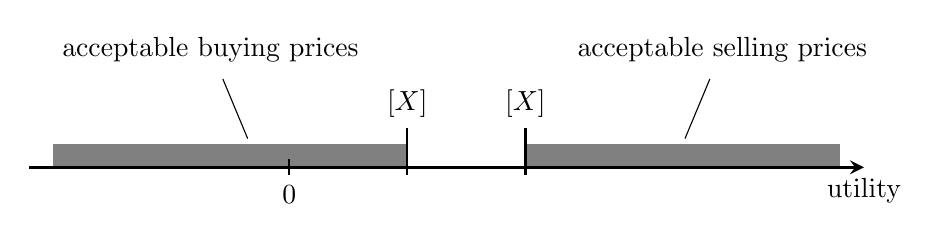
\begin{tikzpicture}[%
linkline/.style={
  shorten >= 2pt,
  shorten <= 3pt
}%
]
\path[fill=gray] (0,0) rectangle (4.5,0.3);
\path[fill=gray] (6,0) rectangle (10,0.3);
\draw[very thick,-stealth] (-0.3,0) -- (10.3,0) node[below] {utility};
\draw[thick] (3,0.1) -- (3,-0.1) node[below] {$0$};
\draw[thick] (4.5,-0.1) -- (4.5,0.5) node[above] {$\El[X]$};
\draw[thick] (6,-0.1) -- (6,0.5) node[above] {$\Eu[X]$};
\node (buy) at (2,1.5) {acceptable buying prices};
\node (sell) at (8.5,1.5) {acceptable selling prices};
\draw[linkline] (buy) -- (2.5,0.3);
\draw[linkline] (sell) -- (8,0.3);
\end{tikzpicture}
\caption{\label{fig:pricesforgambles}%
Illustration of \underline{E} %$\El$ %strange errors occur
and $\Eu$ as supreme buying and infimum selling prices for a gamble $X$ on a linear utility scale.}
\end{figure}

A lower and upper prevision are called \emph{conjugate}%
\footnote{Conjugacy in this sense should not be confused
with conjugacy of prior distributions as discussed in Section~\ref{sec:regularconjugates}.}
if the relation $\Eu[X] = -\El[-X]$ holds for all $X \in \mathcal{K}$.%
\footnote{This implies the relation $\Pl(A^\com) = 1 - \Pu(A)$
of lower and upper probabilities for events $A \subset \Omega$
as mentioned in Section~\ref{sec:ip-general}.}
Then, it suffices to consider only either of $\El$ or $\Eu$,
and in the literature $\El$ is chosen,
the theory consequently being referred to as the theory of
\emph{coherent lower previsions} \parencite[See, e.g.,][Chapter~3.2]{itip}.

Before we explain the concept of \emph{coherence},
the most basic rationality requirement put forward by Walley is
that a lower prevision $\El$ should fulfill the property of
\emph{avoiding sure loss}.
This means that a subject, whose state of information about the
occurence of `states of the world' from the possibility space $\Omega$
is encoded in his or her choice of $\El$,
acting by buying and selling gambles accordingly,
should choose $\El$ such that there is no combination of gambles
%$X_i$, $i=1,\ldots,k$, %of which each is, by $\El$, 
that would result in a net loss, for all $\omega \in \Omega$.

avoiding sure loss --- coherence --- natural extension

epistemic/behavioural



\subsection{Related Concepts}

many links to concepts that aim to complement probability theory as tool for handling uncertainty,
like possibilistic reasoning, fuzzy probabilities, etc.


\section{***Motivations for IP}

Although strictly negated by advocates of Bayesian methods \parencite[e.g., by][]{1987:lindley},
the need to go beyond usual probability measures has been recognized for a long time,%
\footnote{\textcite{2009:hampel} and \textcite[Section~1]{2001:weichselberger} give a historical overview on the development of
ideas related to non-additive measures and interval probability.}
and in recent times most prominently by scientists involved in the development of expert systems.

***klir citation (festschrift)***

\subsection{\pdc }

\subsection{Weakly Informative Priors}


\subsection{Other Motives}

%for later in IDM/IBBM discussion:\\
%we use Walley's \cite[\S 7.7.3, p.~395]{1991:walley} $(s,\vec{t})$ notation for the hyperparameters.
